%%%%%%%%%%%%%%%%%%%%%%%%%%%%%%%%%%%%%%%%%
% Journal Article
% LaTeX Template
% Version 1.4 (15/5/16)
%
% This template has been downloaded from:
% http://www.LaTeXTemplates.com
%
% Original author:
% Frits Wenneker (http://www.howtotex.com) with extensive modifications by
% Vel (vel@LaTeXTemplates.com)
%
% License:
% CC BY-NC-SA 3.0 (http://creativecommons.org/licenses/by-nc-sa/3.0/)
%
%%%%%%%%%%%%%%%%%%%%%%%%%%%%%%%%%%%%%%%%%

%----------------------------------------------------------------------------------------
%	PACKAGES AND OTHER DOCUMENT CONFIGURATIONS
%----------------------------------------------------------------------------------------

\documentclass[twoside,twocolumn]{article}

\usepackage{blindtext} % Package to generate dummy text throughout this template
\usepackage{mathtools}
\usepackage[sc]{mathpazo} % Use the Palatino font
\usepackage[T1]{fontenc} % Use 8-bit encoding that has 256 glyphs
\linespread{1.05} % Line spacing - Palatino needs more space between lines
\usepackage{microtype} % Slightly tweak font spacing for aesthetics

\usepackage{dsfont}
\usepackage[english]{babel} % Language hyphenation and typographical rules

\usepackage[hmarginratio=1:1,top=32mm,columnsep=20pt]{geometry} % Document margins
\usepackage[hang, small,labelfont=bf,up,textfont=it,up]{caption} % Custom captions under/above floats in tables or figures
\usepackage{booktabs} % Horizontal rules in tables

\usepackage{lettrine} % The lettrine is the first enlarged letter at the beginning of the text

\usepackage{enumitem} % Customized lists
\setlist[itemize]{noitemsep} % Make itemize lists more compact
\usepackage{amsmath}
\usepackage{abstract} % Allows abstract customization
\renewcommand{\abstractnamefont}{\normalfont\bfseries} % Set the "Abstract" text to bold
\renewcommand{\abstracttextfont}{\normalfont\small\itshape} % Set the abstract itself to small italic text

\usepackage{titlesec} % Allows customization of titles
\renewcommand\thesection{\Roman{section}} % Roman numerals for the sections
\renewcommand\thesubsection{\roman{subsection}} % roman numerals for subsections
\titleformat{\section}[block]{\large\scshape\centering}{\thesection.}{1em}{} % Change the look of the section titles
\titleformat{\subsection}[block]{\large}{\thesubsection.}{1em}{} % Change the look of the section titles

\usepackage{fancyhdr} % Headers and footers
\pagestyle{fancy} % All pages have headers and footers
\fancyhead{} % Blank out the default header
\fancyfoot{} % Blank out the default footer
\fancyhead[C]{Applied Econometric Policy Evaluation - Spring 2018 - Course notes} % Custom header text
\fancyfoot[RO,LE]{\thepage} % Custom footer text

\usepackage{titling} % Customizing the title section

\usepackage{hyperref} % For hyperlinks in the PDF

%----------------------------------------------------------------------------------------
%	TITLE SECTION
%----------------------------------------------------------------------------------------

\setlength{\droptitle}{-4\baselineskip} % Move the title up

\pretitle{\begin{center}\Huge\bfseries} % Article title formatting
\posttitle{\end{center}} % Article title closing formatting
\title{Advanced Microeconometrics \\ \Large course notes} % Article title
\author{%
\textsc{Kristian Olesen Larsen}\thanks{\href{mailto:kuol@econ.ku.dk}{kuol@econ.ku.dk}. Please share these notes with as many people as you feel like.} \\[1ex] % Your name
\normalsize University of Copenhagen %\\ % Your institution
%\normalsize  % Your email address
%\and % Uncomment if 2 authors are required, duplicate these 4 lines if more
%\textsc{Jane Smith}\thanks{Corresponding author} \\[1ex] % Second author's name
%\normalsize University of Utah \\ % Second author's institution
%\normalsize \href{mailto:jane@smith.com}{jane@smith.com} % Second author's email address
}
\date{\today} % Leave empty to omit a date
\renewcommand{\maketitlehookd}{%
\begin{abstract}
These are my notes for the course Applied Econometric Policy Evaluation. I will attempt to cover each lecture in one or two pages, making reading the whole note-sheet feasible in a few hours.
\end{abstract}
}

%----------------------------------------------------------------------------------------

\begin{document}

% Print the title
\maketitle

%----------------------------------------------------------------------------------------
%	ARTICLE CONTENTS
%----------------------------------------------------------------------------------------

%\section{Introduction}
These course notes are written as part of my personal studies for an exam, and should be taken only to reflect my understanding of the topic. I cannot guarantee that everything in these notes is correct, much less that the explanations provided here are better than those that others have already provided. To fully understand the topics covered i suggest following a similar course yourself.

\tableofcontents

\section{Introduction Lecture}
Frequentist estimators are those most often encountered in undergraduate studies including basic statistics. The term frequentist hints at the estimators utilizing the frequency with which observations appear to estimate underlying models. Extremum estimation is a generalized framework to study these estimators. Common for all extremum estimators is a \textit{stochastic criterion function} $Q_N(\theta)$ which is to be minimized, as well as data $w_i = \{y_i, x_i'\}_{i = 1}^N$. Using these ingredients, as well as a set of assumptions (i.e. $E[\epsilon|x] = 0$) and a parametric representation of the model. An extremum estimator is formally then an estimator which solves
\begin{equation}
\hat{\theta}_{E} = \underset{\theta}{\textrm{arg min }}  Q_N(\theta)
\end{equation}

In these notes all of the frequentist estimators studied will be asymptotically normal, with limit distribution (more on this later)
\begin{equation}
\hat{\theta}_N \overset{a}{\sim} \mathcal{N}(\theta_0, A_0^{-1}B_0 A_0^{-1})
\end{equation}

Usually the two matrices $A_0$ and $B_0$ can be estimated by the hessian and the outer product of the gradients respectively. It is the criterion function $Q_N(\cdot)$ that essentially defines the properties of an estimator. A subgroup of extremum estimators is the M estimators, defined by solving the problem
\begin{equation}
\hat{\theta}_N = \underset{\theta}{\textrm{arg min }} \frac{1}{N} \sum_{i=1}^N q(w_i, \theta)
\end{equation}
In other words M-estimators are extremum estimators where $Q_N(\theta) = \frac{1}{N} \sum_{i=1}^N q(w_i , \theta)$. The advantage to working with M-estimators compared to the more general extremum estimators, is that they allow for the application of a law of large number and the central limits theorem.
\subsection{Identification}
Identification essentially ensures that one can estimate a unique solution for each of the model parameters. Mathematically $\theta_1$ is identified if $P_{\theta_1}(w) = P_{\theta_2}(w), \forall w \in \mathcal{W}$ iff $\theta_1 = \theta_2$. In the case of extremum estimators this is equivalent with the requirement that
\begin{equation}
Q(\theta_0) < Q(\theta), \quad \forall \theta \in \Theta : \theta \neq \theta_0
\end{equation}
In the case of M-estimators this can be reduced to
\begin{equation*}
E[q(w_i,\theta_0)] < E[q(w_i, \theta)], \quad \forall \theta \in \Theta : \theta \neq \theta_0
\end{equation*}

\subsection{Consistency}
Assuming the specified model is correct compared to the underlying datagenerating process (DGP), and thus is identified we can derive consistency on the basis of the criterion function. Consistency is the notion that for large values of the sample size $N$ the estimator should converge in probability to $\theta_0$, formally a convergent estimator $\hat{\theta}_N$ has the property that
\begin{equation}
\textrm{plim } \hat{\theta}_N = \theta_0
\end{equation}
or equivalently
\begin{equation}
\lim_{N \rightarrow \infty} \textrm{Pr}\left(
 |\hat{\theta}_N - \theta_0|> \epsilon
\right)
= 0, \quad \forall \epsilon > 0
\end{equation}
In simple cases, such as for OLS we know how to express the model in simple terms that allow for the derivation of consistency, but in the general case we know nothing else than the criterion function $Q_N(\cdot)$. The concept is illustrated in figure \ref{fig: consistentextremum}.

\begin{figure}
\caption{Concept of consistency in extremum estimators}
\label{fig: consistentextremum}
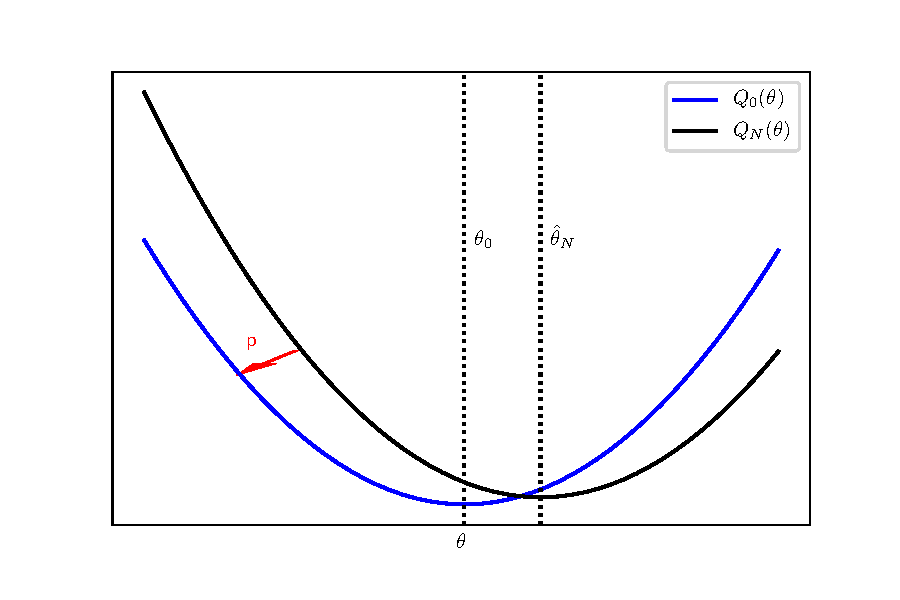
\includegraphics[width = \linewidth]{figures/extremumconv}
\caption*{As $N$ increases consistency will mean for the criterion function $Q_N(\theta)$ to converge in probability to the actual criterion function $Q_0(\theta)$, thus yielding a consistent estimate of $\hat{\theta}_N$.}
\end{figure}

We can think of $Q_N(\cdot)$ as the sample criterion function, which when minimized yields a sample parameter estimate $\hat{\theta}_0$, and likelise the population criterion $Q_0(\cdot)$ yields the true parameter $\theta_0$. The goal in showing consistency is to show that the sample criterion converges in probability to $Q_0(\cdot)$. For M-estimators applying a law of large numbers gives that
\begin{equation}
\frac{1}{N} \sum_{i=1}^N q(w_i, \theta) \underset{N \rightarrow \infty}{\rightarrow} E[q(w_i, \theta)] \equiv Q_0(\theta)
\end{equation}
but this is not possible in the case of extremum estimators. Instead, c.f theorem 5.1 of C\&T the following assumptions will ensure that an estimator $\hat{\theta}_N$ is consistent:
\begin{itemize}
\item The parameter space $\Theta$ is a compact subset of $\mathbb{R}^q$, compact meaning closed an bounded. (Note that $\mathbb{R}$ is not compact, making this asusmptions untrue for most estimation methods in practise).
\item $Q_N(\theta)$ is measurable and continous for all $\theta \in \Theta$.
\item $Q_N(\theta)$ converges uniformly in probability to a nonstochastic function $Q_0(\theta)$, which has a unique global maximum at $\theta_0$.
\end{itemize}
Assuming continuity and measurability of $Q_N(\theta)$ and compactness of $\Theta$ allows to invoke the extreme value theorem, which simply guarantees that a minimum and amaximum of $Q_N(\cdot)$ over a closed interval $[a,b]$ will exist.

\subsection{Asymptotic distribution}
To derive the limit distribution of $\hat{\theta}_N$ we will invoke the \textit{mean value theorem}, which has a very intuitive graphical presentation shown in figure \ref{fig: MVT}. Mathematically we simply equate the derivative of a function, measured in a point $x^+$ with the slope of a line connecting two points $[x_0,x_1]$. To use the theorem it is required that $Q_N(\cdot)$ is twice differentiable around $\theta_0$. Applying the mean value theorem on $\frac{\partial Q_N(\theta)}{\partial \theta}$ on the interval $[\hat{\theta}_N, \theta_0]$ will yield

\begin{multline}
\frac{\partial Q_N(\theta)}{\partial \theta} \bigg{|}_{\hat{\theta}_N} =
\frac{\partial Q_N(\theta)}{\partial \theta} \bigg{|}_{\theta_0} \\ +
\frac{\partial^2 Q_N(\theta)}{\partial \theta \partial \theta'} \bigg{|}_{\theta^+}(\hat{\theta}_N - \theta_0)
\end{multline}

Where by definition $\frac{\partial Q_N(\theta)}{\partial \theta} \bigg{|}_{\hat{\theta}_N} = 0$ so rearranging leaves us with


\begin{multline} \label{eq: asyms}
\sqrt{N}(\hat{\theta}_N - \theta_0) = \left( \frac{\partial^2 Q_N(\theta)}{\partial \theta \partial \theta'} \bigg{|}_{\theta^+} \right)^{-1}  \\ \times
\left(
\frac{\partial Q_N(\theta)}{\partial \theta} \bigg{|}_{\theta_0} \sqrt{N}
\right)
\end{multline}


\begin{figure}
\caption{Mean Value Theorem illustration}
\label{fig: MVT}
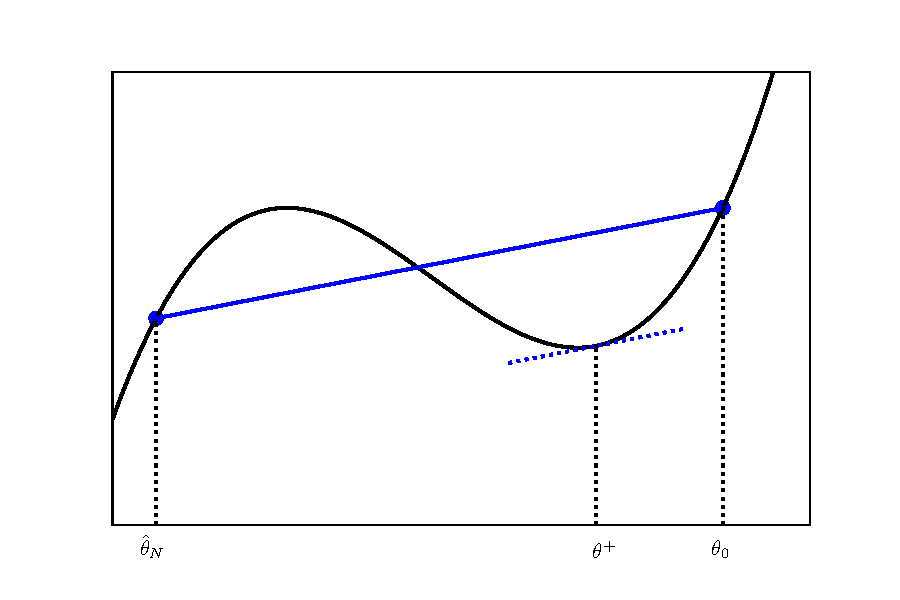
\includegraphics[width = \linewidth]{figures/mvt}
\caption*{The mean value theorem essentially tells us that any continous function $f(z)$ over the interval $\mathcal{I}$ will have at least one point in $\mathcal{I}$ where $\frac{\partial f(z)}{\partial z}$ equals the slope between the endpoints of $\mathcal{I}$.}
\end{figure}

It is then assumed that the following matrices exist and, that the terms converge towards
\begin{align*}
&\frac{\partial^2 Q_N(\theta)}{\partial \theta \partial \theta'} \bigg{|}_{\theta^+} \overset{p}{\rightarrow} A_0 \\
& \frac{\partial Q_N(\theta)}{\partial \theta} \bigg{|}_{\theta_0} \sqrt{N} \overset{d}{\rightarrow} \mathcal{N}(0,B_0)
\end{align*}
If $A_0$ and $B_0$ exist, we can then see from the expression in \eqref{eq: asyms} that asymptotically a consistent M estimator $\hat{\theta}_N$ has distribution
 \begin{equation}
 \sqrt{N}(\hat{\theta}_N - \theta_0) \overset{d}{\rightarrow} \mathcal{N}(0, A_0^{-1}B_0A_0^{-1})
 \end{equation}
In practise of course $A_0$ and $B_0$ are unknown, and will have to be estimated, usually with the following empirical matrices

\begin{align*}
&\hat{A} = \frac{\partial^2 Q_N(\theta)}{\partial \theta \partial \theta'} \bigg{|}_{\hat{\theta}}
\\
& \hat{B} = \frac{1}{N} \sum_{i=1}^N \frac{\partial q(w_i, \theta)}{\partial \theta} \bigg{|}_{\hat{\theta}} \frac{\partial q(w_i, \theta)}{\partial \theta'} \bigg{|}_{\hat{\theta}}
\end{align*}

\subsubsection{Maximum likelihood estimators}
Maximum likelihood estimators has the property that $Q_N(\theta)$ is specified so that
\begin{equation}
Q_N(\theta) = - \sum_{i=1}^N \log L_i(\theta| x_i,y_i)
\end{equation}
Because of this the sandwich expression for the variance derived above collapses to an even simpler expression where $\hat{\theta}_{ML} \sim \mathcal{N}(0, [\mathcal{I}(\theta)]^{-1})$ where $\mathcal{I}(\theta)$ is the fischer information, defined as
\begin{equation}
\mathcal{I}(\theta) = -E\left[ \frac{\partial^2 \log L_i(\theta| x_i,y_i)}{\partial \theta \partial \theta'} \right]
\end{equation}
The proof of this is as follows

Use that $\log L_i(\theta |x_i, y_i) \propto f(y_i | \theta)$, that is the likelihood is proportional to the density of the data. Starting here, we know that
\begin{equation}
\int_{\mathbb{R}} f(y_i | \theta) = 1
\end{equation}
and since the bound of the integral does not depend on $\theta$ taking the derivative w.r.t it on both sides gives
\begin{equation}
\int_{\mathbb{R}} \frac{\partial}{\partial \theta} f(y_i | \theta) = 0
\end{equation}
Now apply that $\frac{\partial \log f(x)}{\partial x} = \frac{\partial f(x)}{\partial x} [f(x)]^{-1}$ to get
\begin{equation}
\int_{\mathbb{R}} \frac{\partial \log f(y_i | \theta)}{\partial \theta}  f(y_i | \theta) = 0
\end{equation}
Using again the rewrite of the derivative of the log of a function gives
\begin{align}
&\int_{\mathbb{R}} \frac{\partial}{\partial \theta} \frac{\partial \log f(y_i | \theta)}{\partial \theta}  f(y_i | \theta) = 0
\end{align}
Which when written out gives
\begin{align*}
 \int_{\mathbb{R}}  &\frac{\partial \log f(y_i | \theta)}{\partial \theta}  \frac{\partial f(y_i | \theta)}{\partial \theta}
\\ &+ \frac{\partial^2 \log f(y_i | \theta)}{\partial \theta \partial \theta'} f(y_i|\theta)
 = 0
\end{align*}
Using the log-derivative trick one final time gives the desired result
\begin{align*}
 \int_{\mathbb{R}}  &\frac{\partial f(y_i | \theta)}{\partial \theta}  \frac{\partial f(y_i | \theta)}{\partial \theta} f(y_i | \theta)
\\ &+ \frac{\partial^2 \log f(y_i | \theta)}{\partial \theta \partial \theta'} f(y_i|\theta)
 = 0
\end{align*}
Or written in terms of expectations
\begin{equation}
E \left[
\frac{\partial f(y_i | \theta)}{\partial \theta}  \frac{\partial f(y_i | \theta)}{\partial \theta}
\right]
= - E\left[
\frac{\partial^2 \log f(y_i | \theta)}{\partial \theta \partial \theta'}
\right]
\end{equation}
Comparing this expression to the $A_0^{-1}B_0A_0^{-1}$ expression derived above should make it clear why the asymptotic variance of maximum likelihood estimators simplifies to the fischer information.


\section{Regression Analysis}
The motivation behind numerical optimization is simple: often we come across functions that are difficult to optimize analytically, and in any case computers are not very good at analytical math. Instead of solving problems exactly, we would like to have methods which come close to the true solution without being to computationally intensive.

In the lectures a host of topics including steepest descent optimization and non-gradient based methods were covered, but here we'll only give a brief overview of the Newton Rhapson algorithm.

\subsection{The Newton Rhapson algorithm}
The idea of the Newton Rhapson algorithm is to intiate the maximization of a function $f(x)$ at some starting guess $x_0$, where a second order Taylor polynomial $p(x_0)$ is constructed. The next point in the procedure will then be the $x=x^1$ where $p(x_1)$ is minimized. The algorithm is generalized to the multivariate case, but the intuition nonetheless remains the same. Let $x_o \in \mathbb{R}^p$ then the second order Taylor approximation of $f(\cdot)$ around $x_0$ is
\begin{multline}
p(x) = f(x_0) + \nabla f(x_0) (x- x_0) \\+ (x-x_0)'\frac{\nabla^2 f(x_0)}{2}(x-x_0)
\end{multline}
for which there is naturally only one solution when solving $p'(x) = 0$, which is the one where
\begin{equation}
x = x_0 - [\nabla^2 f(x_0)]^{-1} \nabla f(x_0)
\end{equation}
This equation gives the next point $x$ to approximate as a function of the current point of approximation $x_0$. It should be noted that the second term is essentially \textit{slope over curvature}. Generalizing the above equation to an iterative algorithm leads to the Newton Rhapson equation
\begin{equation}
x_{n+1} = x_n - s_n [\nabla^2 f(x_n)]^{-1} \nabla f(x_n)
\end{equation}
where $s_n$ is some arbitrarily chosen step size, which ensures the algorithm doesn't get stuck in a steady state, where it jumps back and forth between two suboptimal points.

\subsubsection{Berndt-Hall-Hall-Hausman (BHHH)}
Computationally estimating the hessian at every step might be to costly, so as an alternative the BHHH algorithm utilizes the results derived for ML estimators above, and estimates the hessian as a product of gradients, that is
\begin{equation}
\frac{\partial^2 Q_N(x)}{\partial x \partial x'} \approx \sum_{i=1}^N \frac{\partial q_i(x)}{\partial x} \frac{\partial q_i(x)}{\partial x'}
\end{equation}
with this procedure it is only neccesary to estimate the gradient, which is much less costly than computing the hessian. On the other hand, if the model is wrongly specified, or the sample is small BHHH will perform poorly.


\section{The counterfactual Setup}
Nonlinear least squares is, as the name suggests similar to OLS, but with the added ability to handle nonlinear relations. Before jumping to use NLS, it should however be considered if the relationship of interest is nonlinear even when considering variable transformations. If this not is the case, NLS might be the right choice of estimator. We begin by defining the model, noting that NLS is a M-estimator, due to the form of it's criterion function.

\begin{equation}
y_i = g(x_i, \beta) + u_i, \qquad E[y_i | x_i] = g(x_i, \beta)
\end{equation}
This is very similiar to OLS, but with the addition of a link function $g(\cdot)$, which alters the estimation problem to
\begin{equation}
\hat{\beta}_{NLS} = \underset{\beta}{\textrm{arg max }} \sum_{i=1}^N (y_i - g(x_i, \beta))^2
\end{equation}
Taking the first order conditions is straight forward from here, simply solve $\frac{\partial Q_N(\beta)}{\partial \beta} = 0$. Results on the asymptotic distribution of $\hat{\beta}_{NLS}$ follows from theory on M-estimators.

It can be shown that NLS will be consistent, but not nessecarily efficient if $E[u_i | x_i]=0$, as this assumption alone doesn't account for heteroscedasticity. To account for this, the idea is to implement a weight in the optimization problem. We can show that the optimal weight is the actual variance-covariance matrix $\Omega_0$
\begin{equation}
V[y_i | x_i] = V[u_i|x_i] = E[uu'|x] = \Omega_0
\end{equation}
Of course $\Omega_0$ is unknown, so instead of using this, we begin by simply guessing a matrix $\Sigma$ and estimating $\hat{\beta}_{WNLS}$ as
\begin{equation}
\underset{\beta}{\textrm{arg min }} (y-g(x,\beta))'\Sigma^{-1}(y-g(x,\beta))
\end{equation}
One way to select $\Sigma$ is then to assume that it depends on a set of parameters $\gamma$ and estimate $\hat{\Sigma}=\Sigma(\hat{\gamma})$. In practise this is implemented in steps
\begin{itemize}
\item[1.] Do regular NLS to estimate $\hat{\beta}_{NLS}$
\item[2.] compute the residuals $\hat{u}_i = y_i - g(x_i, \hat{\beta}_{NLS})$ and regress their square on a guessed variance matrix structure and covariates $\gamma$ to get $\hat{\Sigma}$.
\item[3.] Implement the estimated $\hat{\Sigma}$ and conpute the WNLS estimator.
\end{itemize}
This procedure can theoretically be iterated over multiple times, each time refining the estimate of $\hat{\gamma}$ and thus of $\hat{\Sigma}$.



\end{document}
